% =====================================================================
% ch03b.tex —— 第 3 节后半（PDF p.14–19，原书 p.13–18）
% 译者：tr03b；体例见 work/style_guide.md
% 底本：Xi Yin, Aspects of 2D CFTs, PoS(TASI2017)003
% 说明：本片段从 3.2 节（枕形几何与共形块的解析延拓）的续文开始，
%       故不重复 \subsection 标题；随后依次是 3.3、3.4、3.5 三小节。
% =====================================================================

% 衔接说明：上一段末句“而共形块可以看作柱面上的传播子 [11]”已在 ch03a.tex 收句，
% 本片段从 "Its matrix elements are written..." 续译。
其矩阵元写作
\begin{equation}\label{eq:3-27}
  \langle\psi_{43}|q^{L_0-\frac{c}{24}}|\psi_{12}\rangle
  =\sum_{n=0}^{\infty}a_nq^{h+n-\frac{c}{24}},
\end{equation}
其中 $|\psi_{12}\rangle$ 与 $|\psi_{43}\rangle$ 是一对原初场分别插入枕形几何两个角上时生成的态，并投影到权重为 $h$ 的原初场的 Virasoro 后代表示空间；系数 $a_n$ 依赖权重 $h_i$、$h$ 与中心荷 $c$。\eqref{eq:3-27} 与球面四点共形块只差一个共形反常因子：
\begin{equation}\label{eq:3-28}
  \begin{aligned}
  &\mathcal{F}_c(h_1,h_2,h_3,h_4,h;z)\\
  &\quad=\bigl(\theta_3(\tau)\bigr)^{\frac{c}{2}-4(h_1+h_2+h_3+h_4)}
  \,z^{\frac{c}{24}-h_1-h_2}\,(1-z)^{\frac{c}{24}-h_3-h_4}\,
  \langle\psi_{43}|q^{L_0-\frac{c}{24}}|\psi_{12}\rangle .
  \end{aligned}
\end{equation}

% [Tutor Note: \eqref{eq:3-28} 的指数容易记错：$\theta_3$ 上是 $\frac{c}{2}-4(h_1+h_2+h_3+h_4)$，而 $z$、$1-z$ 上是 $\frac{c}{24}-h_i-h_{i+1}$，两处的 $c$ 系数不同（$\frac{c}{2}$ 与 $\frac{c}{24}$），$h_i$ 的系数也不同（$\theta_3$ 上是 4，$z$ 上是 1）。核对时与 \eqref{eq:3-30} 对照，两式的预因子必须逐字相同。]

共形块的枕形表示 \eqref{eq:3-28} 有几条重要性质。第一，\eqref{eq:3-27} 的 $q$ 展开收敛半径为 1，且在去掉原点的单位 $q$ 圆盘上是全纯函数。这覆盖了整个复 $z$ 平面而有余：复 $z$ 平面其实只映到单位 $q$ 圆盘上的一个眼形区域（图~\ref{fig:7}）。第二，矩阵元 \eqref{eq:3-27} 有性质：若取 $h_1=h_4$、$h_2=h_3$，则系数 $a_n$ 是 $|\psi_{12}\rangle$ 的 Virasoro 后代的模方，因而非负（前提是 OPE 与幺正性相容）。

\begin{figure}[htbp]
  \centering
  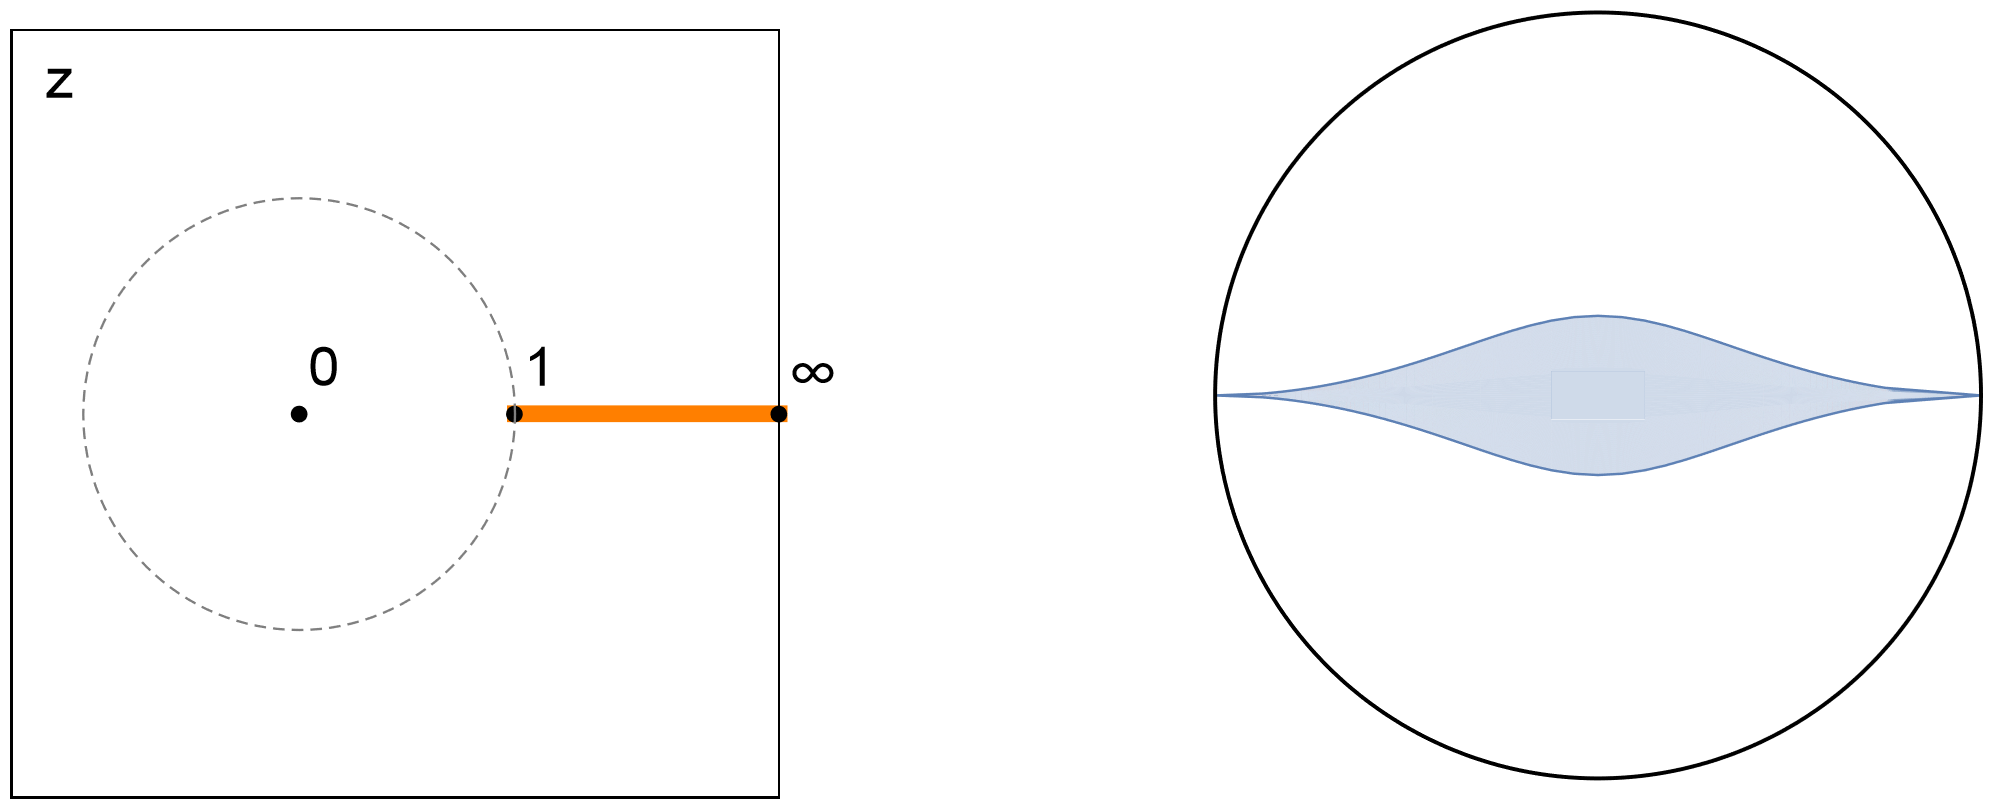
\includegraphics[width=0.85\textwidth]{figures/fig07.png}
  \caption{复 $z$ 平面沿 $[1,\infty)$ 带支割线，映射到单位 $q$ 圆盘上的眼形区域。Virasoro 共形块可解析延拓到整个 $q$ 圆盘。（原文 p.13，图 7）}
  \label{fig:7}
\end{figure}

% [Tutor Note: 图 7 的关键是“映射不覆盖单位 $q$ 圆盘”：$z$ 平面的像只是圆盘内一片眼形区域，两眼尖分别对应 $z=0$ 与 $z=\infty$。正因如此，“$q$ 展开在单位圆盘上收敛”比“$z$ 展开在 $|z|<1$ 收敛”强得多，\eqref{eq:3-28} 才能给出跨过支割线的解析延拓。]

第三，\eqref{eq:3-27} 在 $h\to\infty$ 而 $c$ 与各 $h_i$ 固定的极限下简化：
\begin{equation}\label{eq:3-29}
  \lim_{h\to\infty}\langle\psi_{43}|q^{L_0-\frac{c}{24}}|\psi_{12}\rangle
  =(16q)^{h-\frac{c}{24}}\prod_{n=1}^{\infty}\bigl(1-q^{2n}\bigr)^{-\frac12}.
\end{equation}
从直观上看，大 $h$ 极限下插在角上的外场无关紧要，枕形共形块（至多相差一个与模无关的系数）就等于权重为 $h$ 的原初场环面特征标的平方根。

% [Tutor Note: \eqref{eq:3-29} 里的 $16q$ 是大 $h$ 极限的重标度因子，不能换成 $q$：它来自 $q\to0$ 时 $z=(\theta_2(\tau)/\theta_3(\tau))^4=16q+\cdots$，即 $q$ 与枕形坐标 $z$ 的比值是 16。此式右边的无穷乘积是不含零后代的 Verma 模特征标结构，用来把 \eqref{eq:3-30} 中的 $H_c$ 归一化成 $h\to\infty$ 时趋于 1。]

已知大 $h$ 极限，便可导出以 $h$（而非 $c$）为展开参数的递推公式：
\begin{equation}\label{eq:3-30}
  \begin{aligned}
  \mathcal{F}_c(h_1,h_2,h_3,h_4,h;z)
  &=\bigl(\theta_3(\tau)\bigr)^{\frac{c}{2}-4(h_1+h_2+h_3+h_4)}
  z^{\frac{c}{24}-h_1-h_2}(1-z)^{\frac{c}{24}-h_3-h_4}\\
  &\quad\times(16q)^{h-\frac{c}{24}}
  \prod_{n=1}^{\infty}\bigl(1-q^{2n}\bigr)^{-\frac12}
  H_c(h_1,h_2,h_3,h_4,h;q),
  \end{aligned}
\end{equation}
其中 $H_c$ 满足
\begin{equation}\label{eq:3-31}
  H_c(h_1,h_2,h_3,h_4,h;q)=1+\sum_{r,s\ge1}\frac{q^{rs}}{h-h_{r,s}}\,
  A^c_{rs}P^{rs}_c\begin{bmatrix}h_1\\ h_2\end{bmatrix}
  P^{rs}_c\begin{bmatrix}h_4\\ h_3\end{bmatrix}
  H_c(h_1,h_2,h_3,h_4,h_{r,s}+rs;q).
\end{equation}

% [Tutor Note: \eqref{eq:3-31} 是 Zamolodchikov 的 $h$ 递推（\cite{r10}），与针对 $c$ 的递推 \eqref{eq:3-24} 互为对偶：极点位置由 $c_{r,s}(h)$ 换成 $h_{r,s}(c)$，$A^c_{rs}$ 仍是 \eqref{eq:3-18} 中的量。方括号 $\begin{bmatrix}h_1\\ h_2\end{bmatrix}$ 是对融合矩阵 $P^{rs}_c$ 取相应指标的矩阵元，不是二项式系数。]

实践中可以高效地实现这一递推：先把 \eqref{eq:3-31} 当作线性方程组，对满足 $rs\le n$ 的有限个 $r,s$ 解出 $H_c(h_1,h_2,h_3,h_4,h_{r,s}+rs;q)$ 至 $q^n$ 阶；再用它生成一般内部权重 $h$ 的 $H_c$，同样至 $q^n$ 阶。

\subsection{OPE 的收敛性与交叉方程}

考虑球面四点函数的特例 $\phi_1=\phi_4$、$\phi_2=\phi_3$，它在枕形框架下的共形块分解是求和
\begin{equation}\label{eq:3-32}
  \sum_k C_{12k}^2\,
  \langle\psi^k_{12}|q^{L_0-\frac{c}{24}}|\psi^k_{12}\rangle\,
  \langle\tilde\psi^k_{12}|\bar q^{\bar L_0-\frac{\tilde c}{24}}|\tilde\psi^k_{12}\rangle,
\end{equation}
其中把上标 $k$ 标在 $|\psi^k_{12}\rangle$ 上，用以强调它依赖内部权重 $h_k$。四点函数对 $0<z<1$ 的实 $z$ 解析，故共形块和对 $0<q<1$ 的实 $q$ 收敛；又因 \eqref{eq:3-27} 的系数 $a_n$ 非负，由 Cauchy--Schwarz 不等式即知它对整个 $q$ 圆盘收敛。\eqref{eq:3-32} 的被加项在大内部权重极限下按 $C_{12k}^2(16q)^{h_k+\tilde h_k}$ 增长，于是实 $q$ 接近 1 时的收敛性表明：在单位 $q$ 圆盘内部、$h_*,\tilde h_*\to\infty$ 的极限下，权重 $h_k>h_*$、$\tilde h_k>\tilde h_*$ 的算符对 \eqref{eq:3-32} 的贡献被 $|q|^{h_*+\tilde h_*}$ 压低（若把 $h_k$ 或 $\tilde h_k$ 之一保持在有限区间，可作类似论证）。这一结果说明：枕形框架下 $\phi_1\phi_2$ 的 OPE 作为对内部原初场的求和，以指数式快的速度收敛。

% [Tutor Note: 由实 $q$ 的收敛推出整个 $q$ 圆盘上的收敛，靠的正是 $a_n\ge0$：此时 \eqref{eq:3-27} 呈平方和结构，Cauchy--Schwarz 不等式给出 $q$ 圆盘边界上的收敛性，再作解析延拓。另，原文此处的 “convergences” 应为 “converges”，属语法笔误，不影响数学内容。]

理解共形块展开的收敛性之后，便可把一个一般四点函数 $\langle\prod_{i=1}^4\phi_i(z_i,\bar z_i)\rangle$ 按三种不同通道分解：
\begin{equation}\label{eq:3-33}
  s:\,12\to34,\qquad t:\,14\to23,\qquad u:\,13\to24 .
\end{equation}

% [Tutor Note: \eqref{eq:3-33} 的箭头读作“先对箭头左侧两场作 OPE，再与右侧两场缩并”，即 $s$ 通道配对 $(\phi_1\phi_2)(\phi_3\phi_4)$，$t$ 通道配对 $(\phi_1\phi_4)(\phi_2\phi_3)$。原文只写配对编号，省略了箭头的含义。]

这些共形块分解的等价性给结构常数很强的约束。在外场的各种置换意义下，只需检查 $s$ 通道与 $t$ 通道的等价。把 $z\to1-z$ 并同时交换 $h_1$ 与 $h_3$，便从 $s$ 通道共形块得到 $t$ 通道共形块。两者的等价可写成交叉方程
\begin{equation}\label{eq:3-34}
  \begin{aligned}
  &\sum_k C_{12k}C_{34k}\,
  \mathcal{F}_c(h_1,h_2,h_3,h_4,h_k;z)\,
  \overline{\mathcal{F}}_c(\tilde h_1,\tilde h_2,\tilde h_3,\tilde h_4,\tilde h_k;\bar z)\\
  &\quad=\sum_k C_{14k}C_{23k}\,
  \mathcal{F}_c(h_3,h_2,h_1,h_4,h_k;1-z)\,
  \overline{\mathcal{F}}_c(\tilde h_3,\tilde h_2,\tilde h_1,\tilde h_4,\tilde h_k;1-\bar z).
  \end{aligned}
\end{equation}

% [Tutor Note: \eqref{eq:3-34} 就是二维修正自举的出发点。注意右边第一个共形块的宗量顺序是 $(h_3,h_2,h_1,h_4)$ 而非 $(h_1,h_3,\dots)$：$t$ 通道把 1 与 3 交换，故 1、3 两个位置上的权重随之交换，但 2、4 的位置不动。]

\subsection{交叉方程的解：极小模型}

现在讨论交叉方程最简单的非平凡解之一：$c=\frac12$ 极小模型中非平凡原初场的四点函数。这个模型又称二维临界 Ising 模型。该 CFT 只有三个原初场，权重为
\begin{equation}\label{eq:3-35}
  \begin{aligned}
  1&:\quad h=\tilde h=h_{1,1}=0,\\
  \sigma&:\quad h=\tilde h=h_{1,2}=\frac{1}{16},\\
  \varepsilon&:\quad h=\tilde h=h_{2,1}=\frac12 .
  \end{aligned}
\end{equation}

我们聚焦四点函数 $\langle\sigma(0)\sigma(z,\bar z)\sigma(1)\sigma'(\infty)\rangle\equiv f(z,\bar z)$ 这一例子。$\sigma$ 在能级 2 有一个零后代，形如
\begin{equation}\label{eq:3-36}
  \Bigl(L_{-1}^2-\frac34L_{-2}\Bigr)\sigma
  =\Bigl(\bar L_{-1}^2-\frac34\bar L_{-2}\Bigr)\sigma=0 .
\end{equation}

% [Tutor Note: \eqref{eq:3-36} 的系数 $\frac34$ 来自一般的能级 2 零矢量 $\bigl(L_{-1}^2-\frac{2(2h+1)}{3}L_{-2}\bigr)|h\rangle=0$；代入 $h=h_{1,2}=\frac{1}{16}$ 得 $\frac{2(2h+1)}{3}=\frac34$。这类零矢量沿退化曲线 $h=h_{1,2}(c)$（以及 $h=h_{2,1}(c)$）都存在，$c=\frac12$、$h=\frac{1}{16}$ 只是其中的 Ising 点；正是这类零态使极小模型的共形块可解。]

把 \eqref{eq:3-36} 代入四点函数，得
\begin{equation}\label{eq:3-37}
  \Bigl\langle\sigma(0)\Bigl(L_{-1}^2-\frac34L_{-2}\Bigr)\sigma(z,\bar z)\sigma(1)\sigma'(\infty)\Bigr\rangle=0 .
\end{equation}

作用在 $\sigma(z)$ 上的 $L_{-1}$ 可替换为 $\partial_z$。涉及 $L_{-2}\sigma(z,\bar z)$ 的关联函数用下式计算：
\begin{equation}\label{eq:3-38}
  \begin{aligned}
  &\langle\sigma|\sigma(1)L_{-2}\sigma(z,\bar z)|\sigma\rangle
  =\oint_{C_z}\frac{dw}{2\pi i}\,\frac{1}{w-z}\,
  \langle\sigma|\sigma(1)T(w)\sigma(z)|\sigma\rangle\\
  &\quad=h_{1,2}\Bigl[\frac{1}{(1-z)^2}+\frac{1}{z^2}\Bigr]
  \langle\sigma|\sigma(1)\sigma(z,\bar z)|\sigma\rangle
  -\frac{1}{1-z}\langle\sigma|\partial\sigma(1)\sigma(z,\bar z)|\sigma\rangle
  +\frac1z\langle\sigma|\sigma(1)\sigma(z,\bar z)|\partial\sigma\rangle .
  \end{aligned}
\end{equation}

% [Tutor Note: \eqref{eq:3-38} 第二行的三项分别来自 $T(w)$ 与 $\sigma(1)$、$\sigma(0)$ 的 OPE：$h$ 项给出 $1/(1-z)^2+1/z^2$ 两个双极点，$\partial\sigma(1)$ 与 $\partial\sigma(0)$ 项给出 $-\frac{1}{1-z}$ 与 $+\frac1z$ 两个单极点。末项的 ket $|\partial\sigma\rangle$ 是 $\partial\sigma(0)|0\rangle$ 的简写。核对时注意围道的取向：取向反了会让两个单极点的符号同时翻转。]

涉及 $\partial\sigma$ 的关联函数，可以回到由 $PSL(2,\mathbb{C})$ 不变性确定的一般四点函数形式来计算：
\begin{equation}\label{eq:3-39}
  \langle\sigma(z_1,\bar z_1)\sigma(z_2,\bar z_2)\sigma(z_3,\bar z_3)\sigma'(\infty)\rangle
  =\frac{1}{|z_{31}|^{4h_{1,2}}}\,
  f\Bigl(\frac{z_{21}}{z_{31}},\frac{\bar z_{21}}{\bar z_{31}}\Bigr),
\end{equation}
于是
\begin{equation}\label{eq:3-40}
  \begin{aligned}
  \langle\sigma(0)\sigma(z,\bar z)\partial\sigma(1)\sigma'(\infty)\rangle
  &=\partial_{z_3}\frac{1}{|z_{31}|^{4h_{1,2}}}
  f\Bigl(\frac{z_{21}}{z_{31}},\frac{\bar z_{21}}{\bar z_{31}}\Bigr)
  \Big|_{\substack{z_1=0,\,z_2=z\\ z_3=1}}
  =(-z\partial_z-2h_{1,2})f(z,\bar z),\\
  \langle\partial\sigma(0)\sigma(z,\bar z)\sigma(1)\sigma'(\infty)\rangle
  &=\partial_{z_1}\frac{1}{|z_{31}|^{4h_{1,2}}}
  f\Bigl(\frac{z_{21}}{z_{31}},\frac{\bar z_{21}}{\bar z_{31}}\Bigr)
  \Big|_{\substack{z_1=0,\,z_2=z\\ z_3=1}}
  =\bigl((z-1)\partial_z+2h_{1,2}\bigr)f(z,\bar z).
  \end{aligned}
\end{equation}

% [Tutor Note: 核对 \eqref{eq:3-40} 时用链式法则：全纯部分 $\partial_{z_3}(z_{31})^{-2h_{1,2}}=-2h_{1,2}(z_{31})^{-2h_{1,2}-1}$ 在 $z_3=1$ 处给 $-2h_{1,2}$，而 $\partial_{z_3}(z_{21}/z_{31})=-z$；类似地 $\partial_{z_1}(z_{21}/z_{31})=z-1$、$\partial_{z_1}(z_{31})^{-2h_{1,2}}=2h_{1,2}$。两式合起来把 \eqref{eq:3-38} 中的 $\partial\sigma$ 与 $\partial_z$ 项化到同一个 $f$ 上，再代入 \eqref{eq:3-37} 即得 \eqref{eq:3-41}。]

把 \eqref{eq:3-38} 与 \eqref{eq:3-40} 代入 \eqref{eq:3-37}，得到
\begin{equation}\label{eq:3-41}
  \Bigl[\partial_z^2+\frac{3(1-2z)}{4z(1-z)}\partial_z
  -\frac{3}{64z^2(1-z)^2}\Bigr]f(z,\bar z)=0 .
\end{equation}
此方程有两个线性无关解：
\begin{equation}\label{eq:3-42}
  f_\pm(z)=\frac{\sqrt{1\pm\sqrt z}}{z^{\frac18}(1-z)^{\frac18}} .
\end{equation}

这两个解的线性组合给出两种可能的共形块。此例中只有有限个（即两个）共形块，这是 $\sigma$ 存在零 Virasoro 后代造成的偶然现象。在 $z=0$ 附近展开，得
\begin{equation}\label{eq:3-43}
  \begin{aligned}
  \mathcal{F}_0(z)&=\frac{f_+(z)+f_-(z)}{2}
  =z^{-\frac18}\Bigl(1+\frac{1}{64}z^2+\frac{1}{64}z^3+\frac{117}{8192}z^4+\cdots\Bigr),\\
  \mathcal{F}_{\frac12}(z)&=f_+(z)-f_-(z)
  =z^{\frac38}\Bigl(1+\frac14z+\frac{9}{64}z^2+\frac{25}{256}z^3+\frac{613}{8192}z^4+\cdots\Bigr).
  \end{aligned}
\end{equation}

% [Tutor Note: 展开式的首项指数给出内部权重，$\mathcal{F}_h(z)\sim z^{h-2h_\sigma}$；这里 $2h_\sigma=\frac18$，故 $h=0$ 给 $z^{-1/8}$、$h=\frac12$ 给 $z^{3/8}$，两者指数差 $\frac12=h_\varepsilon$。另，$\mathcal{F}_0$ 展开中 $z^2$ 与 $z^3$ 的系数同为 $\frac{1}{64}$ 并非笔误：$z$ 的一次项在 $f_++f_-$ 中恰好抵消，而 $z^2$、$z^3$ 两项的系数确实相等。]

如记号所示，$\mathcal{F}_h(z)$ 是 $\langle\sigma\sigma\sigma\sigma\rangle$ 中内部原初场权重为 $h$ 的共形块。这里只有单位算符与 $\varepsilon$ 能出现在 $\sigma\sigma$ OPE 中，这是零态微分方程的结果。四点函数因而必取形式
\begin{equation}\label{eq:3-44}
  f(z,\bar z)=\mathcal{F}_0(z)\overline{\mathcal{F}}_0(\bar z)
  +C_{\sigma\sigma\varepsilon}^2\,\mathcal{F}_{\frac12}(z)
  \overline{\mathcal{F}}_{\frac12}(\bar z).
\end{equation}

现在检查交叉对称性：它要求 $f(z,\bar z)$ 在 $z\to1-z$、$\bar z\to1-\bar z$ 下不变。取支割线从 $z=1$ 延伸到 $\infty$，$f_\pm(z)$ 满足
\begin{equation}\label{eq:3-45}
  f_+(1-z)=\frac{f_+(z)+f_-(z)}{\sqrt2},\qquad
  f_-(1-z)=\frac{f_+(z)-f_-(z)}{\sqrt2} .
\end{equation}

% [Tutor Note: \eqref{eq:3-45} 是 $z\to1-z$ 的“单值性字典”，它把绕支点的解析延拓写成两个解之间的正交变换。用它可以把 $\mathcal{F}_0(1-z)$、$\mathcal{F}_{1/2}(1-z)$ 反解成 $\mathcal{F}_0(z)$、$\mathcal{F}_{1/2}(z)$ 的组合：由 $f_\pm=\mathcal{F}_0\pm\frac12\mathcal{F}_{1/2}$ 可得 $\mathcal{F}_0(1-z)=\frac{1}{\sqrt2}\mathcal{F}_0+\frac{1}{2\sqrt2}\mathcal{F}_{1/2}$、$\mathcal{F}_{1/2}(1-z)=\sqrt2\,\mathcal{F}_0-\frac{1}{\sqrt2}\mathcal{F}_{1/2}$。]

于是有
\begin{equation}\label{eq:3-46}
  f(1-z,1-\bar z)
  =\Bigl|\frac{1}{\sqrt2}\mathcal{F}_0+\frac{1}{2\sqrt2}\mathcal{F}_{\frac12}\Bigr|^2
  +C_{\sigma\sigma\varepsilon}^2
  \Bigl|\sqrt2\,\mathcal{F}_0-\frac{1}{\sqrt2}\mathcal{F}_{\frac12}\Bigr|^2 .
\end{equation}

% [Tutor Note: 把 \eqref{eq:3-46} 与 \eqref{eq:3-44} 逐项比较即可定出 $C$：$\mathcal{F}_0\bar{\mathcal{F}}_{1/2}$ 的系数给出 $\frac12-2C^2=0$，即 $C^2=\frac14$；$\mathcal{F}_0\bar{\mathcal{F}}_0$ 与 $\mathcal{F}_{1/2}\bar{\mathcal{F}}_{1/2}$ 的系数给出同一条件。可见交叉对称性把 $C$ 唯一确定为 $\frac12$（符号取正由幺正性）。]

可见交叉对称性成立当且仅当
\begin{equation}\label{eq:3-47}
  C_{\sigma\sigma\varepsilon}=\frac12 .
\end{equation}

事实上，$C_{\sigma\sigma\varepsilon}$ 是 $c=\frac12$ 极小模型中唯一的非平凡结构常数：用类似的分析可证 $C_{\varepsilon\varepsilon\sigma}$ 与 $C_{\varepsilon\varepsilon\varepsilon}$ 都为零。该 CFT 由此完全解出。

还有一组一致性条件必须满足，即原初场环面一点函数的模协变性。它对 $c=\frac12$ 极小模型确实成立，但此处不作显式验证。

% [Tutor Note: 这里说的“模协变性”指环面一点函数在 $SL(2,\mathbb{Z})$ 下的变换性质；极小模型的各原初场都对应已知的模不变配分函数组合，故该条件是自动的。作者略去验证，是因为它不影响球面四点函数的解。]

\subsection{交叉方程的解：Liouville 理论}

现在描述交叉方程的另一个非平凡解。考虑中心荷 $c>1$ 的幺正 CFT，并假设其中只有标量 Virasoro 原初场。假设 $c>1$，是为了让零的 Virasoro 后代不可能出现。要求所有 Virasoro 原初场都是标量，即 $h=\tilde h$，是极强的条件；事实上，这一条件（在猜想意义上）完全固定了该 CFT！

先考察这种 CFT 的环面配分函数，它必须模不变。其一般形式为
\begin{equation}\label{eq:3-48}
  Z(\tau,\bar\tau)=\sum_{h,\tilde h}d_{h,\tilde h}\,
  \chi_h(\tau)\bar\chi_{\tilde h}(\bar\tau),
\end{equation}
其中 $d_{h,\tilde h}$ 是权重为 $(h,\tilde h)$ 的原初场个数，$\chi_h$ 是权重为 $h$ 的原初场的 Virasoro 表示的环面特征标，
\begin{equation}\label{eq:3-49}
  \chi_h(\tau)=\mathrm{Tr}_{\mathcal{V}_h}\,q^{h-\frac{c}{24}},
\end{equation}
其中 $q=e^{2\pi i\tau}$，$\mathcal{V}_h$ 是 $v_h$ 的 Virasoro 后代构成的空间。没有零后代时（$c>1$ 且 $h\ge0$ 保证这一点），有
\begin{equation}\label{eq:3-50}
  \chi_h(\tau)=q^{h-\frac{c}{24}}\prod_{n=1}^{\infty}\frac{1}{1-q^n}.
\end{equation}

% [Tutor Note: \eqref{eq:3-49} 的迹是 $L_0-\frac{c}{24}$ 的指数；\eqref{eq:3-50} 中每个因子 $1/(1-q^n)$ 对应 $L_{-n}$ 取任意次幂。若 $c\le1$ 或 $h<0$，Verma 模含零后代，必须逐个扣除，此式不再成立。还要注意约定：本小节（环面）用 $q=e^{2\pi i\tau}$，而上一小节枕形框架用 $q=e^{i\pi\tau}$，两处的 $q$ 不能混用。]

暂时设 $\tilde c=c$，于是反全纯 Virasoro 特征标就是 $\chi_{\tilde h}$ 的复共轭。模不变性等价于
\begin{equation}\label{eq:3-51}
  Z(\tau,\bar\tau)=Z(\tau+1,\bar\tau+1)=Z(-1/\tau,-1/\bar\tau).
\end{equation}

第一个等式等价于对所有原初场 $h-\tilde h\in\mathbb{Z}$，即自旋为整数。若只有标量原初场（$h=\tilde h$），这一点自然满足。对第二个等式，把配分函数写成
\begin{equation}\label{eq:3-52}
  Z(\tau,\bar\tau)=\frac{1}{|\eta(\tau)|^2}
  \sum_h d_h\exp\Bigl[-4\pi\tau_2\Bigl(h-\frac{c-1}{24}\Bigr)\Bigr],
\end{equation}
再利用 $\eta$ 函数的模性质 $\eta(-1/\tau)=\sqrt{-i\tau}\,\eta(\tau)$，配分函数的模不变性便可写成
\begin{equation}\label{eq:3-53}
  \frac{1}{|\tau|}\sum_h d_h
  \exp\Bigl[-4\pi\frac{\tau_2}{|\tau|^2}\Bigl(h-\frac{c-1}{24}\Bigr)\Bigr]
  =\sum_h d_h\exp\Bigl[-4\pi\tau_2\Bigl(h-\frac{c-1}{24}\Bigr)\Bigr].
\end{equation}

% [Tutor Note: \eqref{eq:3-52} 的 $c-1$ 是这样来的：由 $\eta(\tau)=q^{1/24}\prod(1-q^n)$ 得 $\prod_n(1-q^n)^{-1}=q^{-1/24}/\eta$，故 $\chi_h=q^{h-c/24}\prod(1-q^n)^{-1}=q^{h-(c-1)/24}/\eta$，指数里便出现 $h-\frac{c-1}{24}$，而不是 $h-\frac{c}{24}$。又在取模方时 $|q^{h-(c-1)/24}|^2=e^{-4\pi\tau_2(h-(c-1)/24)}$，其中用到 $\tau_2=\mathrm{Im}\,\tau$。]

为看得更清楚，定义
\begin{equation}\label{eq:3-54}
  x=\tau_2,\qquad y=\frac{\tau_2}{|\tau|^2},
\end{equation}
并把上式写成
\begin{equation}\label{eq:3-55}
  \sqrt{y}\sum_h d_h\exp\Bigl[-4\pi y\Bigl(h-\frac{c-1}{24}\Bigr)\Bigr]
  =\sqrt{x}\sum_h d_h\exp\Bigl[-4\pi x\Bigl(h-\frac{c-1}{24}\Bigr)\Bigr].
\end{equation}

% [Tutor Note: 由 $y=\tau_2/|\tau|^2$ 与 $x=\tau_2$ 得 $|\tau|^2=x/y$，故 $\frac{1}{|\tau|}=\sqrt{y/x}$；\eqref{eq:3-53} 两边同乘 $|\tau|=\sqrt{x/y}$ 即得 \eqref{eq:3-55}，这一步只是变量替换，没有额外假设。]

显然，这只有在两边都与 $x$、$y$ 无关时才可能，即
\begin{equation}\label{eq:3-56}
  \sum_h d_h\exp\Bigl[-4\pi x\Bigl(h-\frac{c-1}{24}\Bigr)\Bigr]\propto x^{-\frac12}.
\end{equation}

对离散的原初场谱，这实际上不可能。我们需要的是权重 $h\ge\frac{c-1}{24}$ 的一族连续原初场，并把求和换成带谱密度 $\rho(h)$ 的积分：
\begin{equation}\label{eq:3-57}
  \sum_h d_h\to\int_{\frac{c-1}{24}}^{\infty}dh\,\rho(h),
\end{equation}
其中
\begin{equation}\label{eq:3-58}
  \rho(h)\propto\frac{1}{\sqrt{h-\frac{c-1}{24}}}.
\end{equation}

% [Tutor Note: 从 \eqref{eq:3-56} 到 \eqref{eq:3-58} 用的是 Laplace 变换：若 $\int_{h_0}^{\infty}dh\,\rho(h)e^{-4\pi x(h-h_0)}\propto x^{-1/2}$，由 $\int_0^{\infty}dt\,t^{-1/2}e^{-4\pi xt}=\Gamma(\frac12)(4\pi x)^{-1/2}$ 即知 $\rho(h)\propto(h-h_0)^{-1/2}$，$h_0=\frac{c-1}{24}$。离散谱之所以不行，是因为有限项指数和在大 $x$ 时按 $e^{-4\pi x\,\Delta}$ 衰减，不可能给出幂律 $x^{-1/2}$。]

若写 $c=1+6Q^2$、$h=\frac{Q^2}{4}+P^2$，则
\begin{equation}\label{eq:3-59}
  \int_{\frac{c-1}{24}}^{\infty}dh\,\rho(h)\propto\int_0^{\infty}dP .
\end{equation}
由此可知，原初场的谱密度对参数 $P$ 必须是平坦分布。

% [Tutor Note: \eqref{eq:3-59} 的下限 $\frac{c-1}{24}=\frac{6Q^2}{24}=\frac{Q^2}{4}$ 正是 $h=\frac{Q^2}{4}+P^2$ 在 $P=0$ 处的值；又 $dh=2P\,dP$，而 \eqref{eq:3-58} 给 $\rho\propto(h-\frac{Q^2}{4})^{-1/2}=1/P$，两者相乘恰好给出平坦的 $dP$ 测度，这就是 \eqref{eq:3-59} 的来历。]

假设没有更多简并，于是标量原初场由 $P$ 标记，记作 $V_P$。两点函数自然归一化为
\begin{equation}\label{eq:3-60}
  \langle V_P(1)V_{P'}(0)\rangle=\delta(P-P').
\end{equation}
结构常数现在是三变量的对称函数 $C(P_1,P_2,P_3)$，OPE 取形式
\begin{equation}\label{eq:3-61}
  V_{P_1}(z,\bar z)V_{P_2}(0)\sim\int_0^{\infty}dP_3\,
  C(P_1,P_2,P_3)\,|z|^{-\frac{Q^2}{2}-2P_1^2-2P_2^2+2P_3^2}
  V_{P_3}(0),
\end{equation}
再加上 Virasoro 后代的贡献。

% [Tutor Note: \eqref{eq:3-61} 的指数可用 $\Delta_i=\frac{Q^2}{4}+P_i^2$ 核对：OPE 系数应为 $|z|^{2(\Delta_3-\Delta_1-\Delta_2)}=|z|^{-Q^2/2-2P_1^2-2P_2^2+2P_3^2}$，注意先算 $2(\Delta_3-\Delta_1-\Delta_2)$，容易漏掉 $Q^2$ 项。]

就球面关联函数而言，关键的一致性条件是交叉方程
\begin{equation}\label{eq:3-62}
  \begin{aligned}
  &\int_0^{\infty}dP\,C(P_1,P_2,P)C(P_3,P_4,P)
  \Bigl|\mathcal{F}_c\Bigl(h_1,h_2,h_3,h_4,h=\frac{Q^2}{4}+P^2;z\Bigr)\Bigr|^2\\
  &\quad=\int_0^{\infty}dP\,C(P_3,P_2,P)C(P_1,P_4,P)
  \Bigl|\mathcal{F}_c\Bigl(h_3,h_2,h_1,h_4,h=\frac{Q^2}{4}+P^2;1-z\Bigr)\Bigr|^2 .
  \end{aligned}
\end{equation}

% [Tutor Note: 与 \eqref{eq:3-34} 相比，连续谱的交叉方程把对 $k$ 的求和换成 $\int_0^{\infty}dP$，并对每个共形块取模方：左右两侧共用同一个内部参数 $P$，不是把两个不同 $P$ 的块相乘。权重 $\frac{Q^2}{4}+P^2$ 对 $P$ 与 $-P$ 相同，故积分只取 $P\ge0$。]

是否存在实值函数 $C(P_1,P_2,P_3)$，使该方程对一切 $P_i$ 都成立？值得注意的是，答案是肯定的，而且解看起来唯一（至多相差一个整体常数倍）。该解称为 Dorn--Otto--Zamolodchikov--Zamolodchikov（DOZZ）结构常数，由下式给出 \cite{r12,r13,r14,r15}：
\begin{equation}\label{eq:3-63}
  C(P_1,P_2,P_3)
  =\frac{\Upsilon_b'(0)}{\Upsilon_b\bigl(\frac{Q}{2}+i(P_1+P_2+P_3)\bigr)}
  \prod_{j=1}^{3}
  \frac{\sqrt{\Upsilon_b(2iP_j)\Upsilon_b(-2iP_j)}}
  {\Upsilon_b\bigl(\frac{Q}{2}+i(P_1+P_2+P_3-2P_j)\bigr)},
\end{equation}
其中 $\Upsilon_b(x)$ 是 Barnes 双重 Gamma 函数，定义为下式从区域 $0<\mathrm{Re}(x)<Q$ 出发的解析延拓：
\begin{equation}\label{eq:3-64}
  \Upsilon_b(x)=\exp\Biggl\{
  \int_0^{\infty}\frac{dt}{t}
  \Biggl[\Bigl(\frac{Q}{2}-x\Bigr)^2e^{-t}
  -\frac{\sinh^2\bigl[\bigl(\frac{Q}{2}-x\bigr)\frac{t}{2}\bigr]}
  {\sinh\frac{tb}{2}\,\sinh\frac{t}{2b}}\Biggr]\Biggr\}.
\end{equation}

% [Tutor Note: \eqref{eq:3-63} 分子里 $\sqrt{\Upsilon_b(2iP_j)\Upsilon_b(-2iP_j)}$ 的写法与多数文献的 DOZZ 形式（分子直接写 $\Upsilon_b(2\alpha_j)$，$\alpha_j=\frac{Q}{2}+iP_j$）不同；由 \eqref{eq:3-65} 的反射关系有 $\Upsilon_b(2\alpha_j)=\Upsilon_b(Q+2iP_j)=\Upsilon_b(-2iP_j)$。两种写法至多相差一个由 $\Upsilon_b(2iP_j)$ 决定的因子，引用别的归一化时务必核对。]

% [Tutor Note: \eqref{eq:3-64} 的积分表示有收敛域限制：$t\to\infty$ 时 $\sinh^2$ 之比趋于 $e^{-xt}$，被积函数按 $e^{-xt}$ 衰减；$t\to0$ 时方括号内两项的领头阶相互抵消，积分才在原点附近有限。作者先在 $0<\mathrm{Re}(x)<Q$ 内定义它，再解析延拓成整函数。]

对一般的 $b$，$\Upsilon_b(x)$ 是复 $x$ 平面上的整解析函数，其单零点位于 $x=mb+n/b$，其中整数 $m,n\le0$ 或 $m,n\ge1$。另外几条有用的性质是
\begin{equation}\label{eq:3-65}
  \begin{aligned}
  \Upsilon_b(Q-x)&=\Upsilon_b(x),\\
  \Upsilon_b(x+b)&=\gamma(bx)\,b^{1-2bx}\,\Upsilon_b(x),\\
  \Upsilon_b(x+b^{-1})&=\gamma(b^{-1}x)\,b^{\frac{2x}{b}-1}\,\Upsilon_b(x),
  \end{aligned}
\end{equation}
其中 $\gamma(x)\equiv\Gamma(x)/\Gamma(1-x)$。

% [Tutor Note: \eqref{eq:3-65} 的三行分别给出关于 $Q/2$ 的对称性与沿 $b$、$1/b$ 两个方向的平移规律；零点位置 $x=mb+n/b$（$m,n\le0$ 或 $m,n\ge1$）正是 \eqref{eq:3-63} 分母中 $\Upsilon_b$ 的零点所在，因此 DOZZ 结构常数只在融合规则允许的取值处出现奇点。]

事实表明，取这组结构常数时，环面一点函数的模协变性也得到满足 \cite{r16}。只含标量原初场的谱连同 DOZZ 结构常数，定义的就是所谓的 Liouville CFT \cite{r15,r17}。


